\documentclass[titlepage]{article}

\usepackage[utf8]{inputenc}
\usepackage[dvipsnames]{xcolor}
\usepackage{amsmath}
\usepackage{tcolorbox}
\usepackage{amssymb}
\usepackage{amsthm}
\usepackage{proof}
\usepackage{float}
\newcommand\blfootnote[1]{%
  \begingroup
  \renewcommand\thefootnote{}\footnote{#1}%
  \addtocounter{footnote}{-1}%
  \endgroup
}
\usepackage{listings}
\lstset{
  basicstyle=\ttfamily,
  mathescape
}



\theoremstyle{definition}


\usepackage[
top    = 2.50cm,
bottom = 2.50cm,
left   = 2.75cm,
right  = 2.75cm]{geometry}
\usepackage{fancyhdr}
\pagestyle{fancy}
\lhead{Advanced computation}
\rhead{EPFL/Alp Ozen}
\newcommand{\floor}[1]{\lfloor #1 \rfloor}

\title{\textbf{Advanced Computation 1 / CS 101}}
\author{Alp Ozen}
\date{Fall 2019}
\newtheorem{theorem}{Theorem}[section]
\newtheorem{example}{Example}
\newtheorem{remark}{Remark}
\newtheorem{definition}{Definition}
\numberwithin{equation}{subsection}
\numberwithin{remark}{subsection}
\newtheorem{question}{Question \textit{?}}[subsection]
\newtheorem{answer}{Answer}[subsection]
\begin{document}

\maketitle

\tableofcontents

\\
    \blfootnote{! Notes \textcolor{gray}{starting in gray} and \textcolor{gray}{ending with grey} are from Prof.Lenstra's own lecture notes.}


\clearpage

\section{Propositional logic and notions of sets(Week 1 - Week 4)}
\subsection{Propositions}
A proposition is a declarative sentence that is either true or false. 
\begin{tcolorbox}
How much does it cost? \textbf{is not a proposition}
\\
I like red \textbf{is a proposition}
\end{tcolorbox}

To make life easier, we represent propositional statements through letters such as $p$. 
\\

The conditional statement $p\implies q$ appears very often. Thus, we have the \textit{converse,contrapositive and inverse} which are:
\\
\textbf{converse}: $q \implies p$
\\
\textbf{contrapositive}: $ \neg q \implies \neg p $
\\
\textbf{inverse}: $ \neg p \implies \neg q$
\\

We note that a conditional is logically equivalent to its contrapositive. 

\begin{tcolorbox}
\centering
\begin{array}{cccccc}
 p & q & p $\implies$ q & \neg q & \neg p & \neg q $\implies$ \neg p \\
 \hline
t & t & t & f & f & t\\
t & f & f & t & f & f\\
f & t & t & f & t & t\\
f & f & t & t & t & t
\end{array}
\end{tcolorbox}

\subsection{Precedence of logical operators}

\begin{figure}[h]
    \centering
    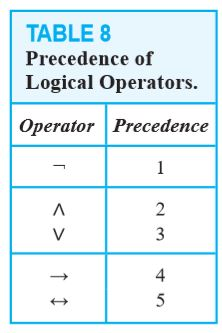
\includegraphics{figures/precedence}
\end{figure}

\subsection{Fuzzy logic}

In fuzzy logic, truth values are between 0 and 1. So if the statement "I like riding a bike" has a value of 0.8, it's negation has 1 minus this value, in this case -0.2. 

\subsection{Applications of logic}
\subsubsection{Logic gates}
Here are the basic logic circuits from which more complex circuits are made: 

\begin{figure}[h]
    \centering
    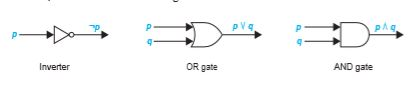
\includegraphics[scale= 1]{epflLectureNotes/advancedComputation/figures/logicgates.JPG}
    \caption{Logic gates}
    \label{fig:my_label}
\end{figure}

Note that the OR and AND gates accept only and only 2 inputs and output one. This input may be as compounded as possible but not exceed 'two chunks'. Thus, when given a complex logical output and reverse engineering, we identify the outer most outer operation, branch it into two or one(if it is simply a negation) and so on. 

\subsubsection{More on propositions}

\begin{tcolorbox}
\begin{itemize}
    \item \textbf{Tautology} is a compound proposition that is always true regardless of the truth value of its variables
    \item \textbf{Contradiction} is a compound proposition that is always false regardless of the truth value of its variables 
    \item \textbf{Contingency} compound statement that is neither tautology nor contradiction
    
    \begin{example}
    \\
    $p \land \neg p$ is a contradiction
    \\
    $p \lor \neg p$ is a tautology
    \end{example}
\end{itemize}
\end{tcolorbox}

Here are some examples of logical calculus:
\\
Show that $\neg(p \lor (\neg p \land q )) \equiveq \neg p \land \neg q$
\begin{align*}
    \neg(p\lor\neg p \land p \lor q)\\
    \neg(T \land p \lor q)\\
    \neg(p \lor q)\\
    \neg p \land \neg q
\end{align*}

\subsubsection{Satisfiability}

A compound proposition is \textbf{satisfiable} if a truth assignment can be made to its variables that make it true making it either a tautology or a contingency. It is \textbf{unsatisfiable} if the negation of the compound statement is a contradiction. 

\subsection{Logical calculus and useful equivalences}

\begin{definition}
If $A \iff B$ is a tautology, then A is logically equivalent to B. 
\end{definition}
\\

Here are some useful logical equivalences(omitting most obvious ones):

\begin{align*}
    p \implies q \equiv \neg p \lor q \equiv \neg(\neg q \lor p) \equiv \neg(q \implies p) \equiv \neg q \implies \neg p \\
    p \lor ( q \land r) \equiv (p \lor q) \land (p \lor r) \\
    \land \ \text{distributes over} \lor \text{and vice versa}\\
    p \lor \neg p \equiv T\\
    p \land \neg p \equiv F\\
    P \land T \equiv p\\
    p \lor F \equiv p
    \ \text{both $\land$ and $\lor$ are associative}
\end{align*}

For more see this figure:

\begin{figure}[h]
    \centering
    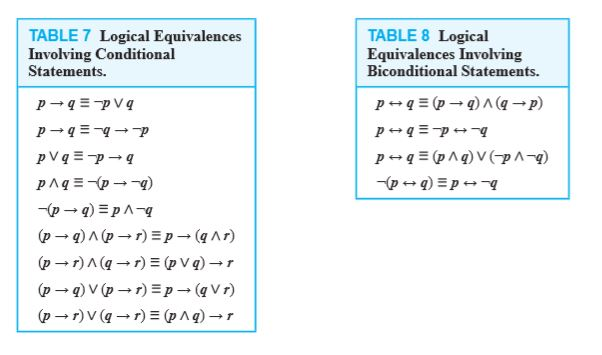
\includegraphics[scale = 0.7]{epflLectureNotes/advancedComputation/figures/logic.JPG}
    \caption{Logic, yey!}
    \label{fig:my_label}
\end{figure}

\begin{definition}
A \textbf{rule of inference} is based on the tautology $p \land (p \implies q) \implies q$. That is, whenever we are given that both $p$ and $p \implies q$ is true, we infer that q must be true. That is :
\\

\infer{q}{p & (p \implies q)}
\end{definition}

Another important fact of logic is that we may boil down all of $\lor, \oplus, \implies, \iff$ to simply propositions involving$\neg, \land$: 

\begin{align*}
    p \lor q \equiv \neg \neg (p \lor q) \equiv \neg(\neg p \land \neg q)\\
    p \oplus q \equiv \neg(p \land q) \land (p \lor q)\\
    p \implies q \equiv \neg p \lor q \equiv \neg (p \land \neg q)\\
    p \iff q \equiv \neg(\neg(p\land q) \land (\neg (\neg p \land \neg q))
\end{align*}


\begin{question}
Given propositional variables and truth values of the single variables for which the compound proposition takes a value, is there a way of deducing a compound proposition? 
\end{question}
\newpage
\subsection{Lec.03 notes}

The \textbf{contrapositive} is the following statement:
\begin{align*}
    p \implies q \equiv \neg p \lor q\\
    \equiv q \lor \neg p\\
    \equiv \neg q \implies \neg p\\
    \therefore p \implies q \equiv \neg q \implies \neg p
\end{align*}
\\
Some useful logical equivalences involving implication:

\begin{align*}
    (p \implies q) \land (p \implies r) \equiv (\neg p \lor q) \land (\neg p \lor r)\\
    \equiv \neg p \lor (q \land r) \equiv p \implies (q \land r)
\end{align*}
And here's a more trivial one: 
\begin{align*}
    (p \implies q) \lor (p \implies r) \equiv (\neg p \lor q) \lor (\neg p \lor r)\\
    \equiv \neg p \lor \neg p \lor q \lor r \equiv \neg p \lor (q \lor r)\\
    \equiv p \implies (q \lor r)
\end{align*}
And slightly more complicated involving De Morgan:
\begin{align*}
    (p \implies r) \land (q \implies r) \equiv (\neg p \lor r) \land (\neg q \lor r)\\
    \equiv \neg r \lor (\neg p \land \neg q) \equiv \neg r \lor (\neg(p \lor q)\\
    \equiv (p \lor q) \implies r 
\end{align*}

We must also add some comments on base b systems of numbers and a general algorithm for conversion. Let's take an example in base 5. Suppose we want to convert $60_{10}$ to its base 5 representation. Well the largest power of 5 less than or equal to 60 is 25 and thus we know that 60 can be \textbf{uniquely} represented as a linear combination of the powers of 5 less than or equal to it. In fact, using powers of 5 less than or equal to 60, we may represent all numbers up to $5^k - 1$ as $4\cdot5^{k-1} + \ldots + 4\cdot5^{0}$. Thus, to represent some $l$ in base $b$ the algorithm is to find the largest power of $b^k < l$, perform $\floor{\frac{l}{b^k}}$ then repeat step 1 and proceed as $l - b^k\cdot\floor{\frac{l}{b^k}}$ and repeat until $l - b^i\cdot\floor{\frac{l}{b^i}} = 0$
 
\subsection{Lec.04 notes}
\subsubsection{More on CMOS}
This was a lecture with a steep curve and here is a summary. First of all, we first revisit some of the concepts of the pmos and nmos resistors. A very important convention is that pmos must never be used for pull-down(connected to GND) and nmos never used for pullup(connected to VDD). 

\begin{figure}[h]
    \centering
    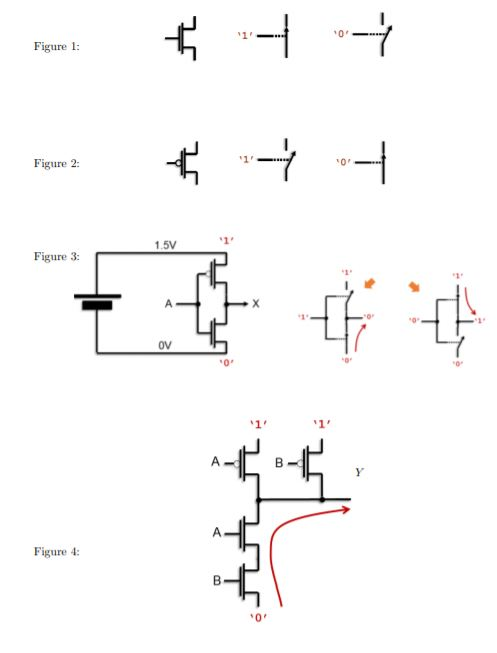
\includegraphics[scale=0.7]{epflLectureNotes/advancedComputation/figures/cmos.JPG}
    \caption{Caption}
    \label{Nmos,Pmos,Inverter,Nand}
\end{figure}

\begin{tcolorbox}
Some principles of cmos gates: 
\begin{itemize}
    \item Pmos goes to top, nmos to bottom.
    \item Never connect high voltage to low voltage to prevent a short circuit. 
    \item Any circuit may be realized as a combination of the NAND and NOR ciruit. 
    \item Each pmos must connect to an nmos. 
\end{itemize}
\end{tcolorbox}
\\
The most challenging part of CMOS circuits is the circuit analysis itself. Consider this example to see a method of circuit analysis: 


\begin{figure}[h!]
    \centering
    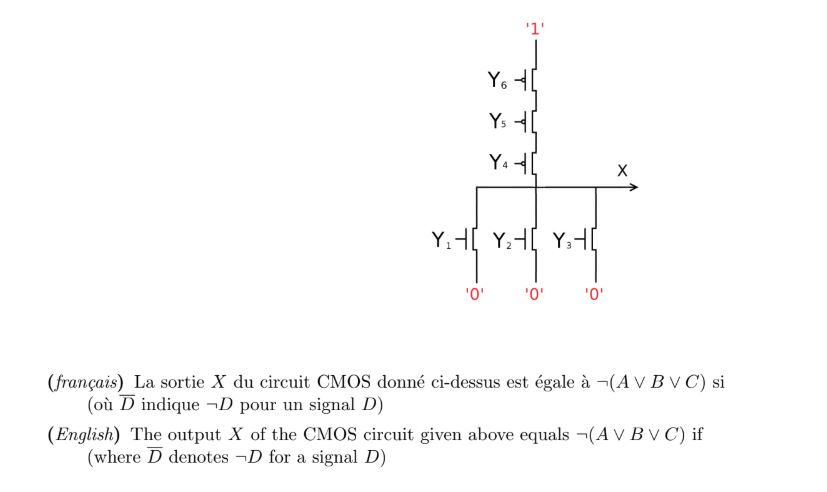
\includegraphics[scale = 0.6]{epflLectureNotes/advancedComputation/figures/cmosq.JPG}
    \caption{exam question}
    \label{exam question}
\end{figure}

\FloatBarrier

\begin{tcolorbox}
Now, first of all, realize that X is connected to VDD iff all of $Y_{6} \land Y_{5} \land Y_{4}$ are grounded. That is $Y_{6} \land Y_{5} \land Y_{4} = 0$. For symbolic purposes, supposing that $Y_{i} = 0 \equiv \neg Y_{i} $ we get that $X = 1 \iff \neg (Y_{4} \lor Y_{5} \lor Y_{6})$ Now given that this is a CMOS circuit, we know that the bottom part does the exact opposite of the upper part. Thus, we have that $X=0 \iff \neg(\neg (Y_{4} \lor Y_{5} \lor Y_{6})) = Y_{4} \lor Y_{5} \lor Y_{6} \equiv Y_{1} \lor Y_{2} \lor Y_{3}$. As a final step, for $\neg (A \lor B \lor C)$ to be true, we need that the output equals $\neg(A \lor B \lor C)$ and since $X=1 \iff \neg (Y_{4} \lor Y_{5} \lor Y_{6})$ we get that $Y_{1} = Y_{2} \ldots$

\end{tcolorbox}

\subsubsection{Binary addition circuit}

Given that we can construct any compound logical gate using CMOS, suppose we want to implement a binary addition calculator. Now here are all the possible cases for doing binary addition: 

\begin{figure}[h]
    \centering
    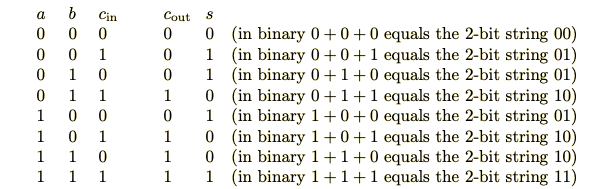
\includegraphics[scale = 0.6]{epflLectureNotes/advancedComputation/figures/binary.png}
    \caption{Addition possibilities}
    \label{fig:my_label}
\end{figure}

Now suppose we want a function $f(a,b,c_{in})$ to evaluate $s$. Well notice that $s$ is only true when the parity of $a,b,c_{in}$ is odd. That is, we may describe this outcome with the function $a \oplus b \oplus c_{in}$. Similarly, devising $g(a,b,c_{in})$ to compute $c_{out}$ we notice that $c_{out}$ evaluates to 1 iff at least two variables are true. This is equivalent to $(a\land b) \lor (a \land c_{in}) \lor (b \land c_{in})$

\subsubsection{Fast Multiplication aka. Karatsuba}
We now ponder whether there is a quick way of multiplying some $v$ and $w$. Now notice that for $v$ and $w$ in base 10, $v = aX + b$ and $w = cX + d$. Now notice that $v \cdot w = (aX+b)(cX+d)$ which in turn is:

\begin{equation*}
    v\cdot w = acX^2 + (ad + bc)X + bd
\end{equation*}

And further notice that:

\begin{equation*}
    ad + bc = (ac + bd) - (a - b)(c - d) 
\end{equation*}

to get:

\begin{equation*}
    v\cdot w = acX^2 + ((ac + bd) - (a - b)(c - d))X + bd
\end{equation*}

Now if for instance $v$ and $w$ were 2 digit numbers, we would normally perform 4 digit by digit multiplications but with this new method, we end up performing only 3 and a trivial subs traction. 
\\
As a general result, for multiplication of two k by k digit numbers, we end up performing $3^{\log_{2}k}$ multiplications and $log_{2}k$ many additions. Finally, notice that Karatsuba is a recursive algorithm. 
\subsubsection{Two's compliment}
Consider how a computer is to represent negative integers. A very smart way of doing so is \textbf{two's compliment}. That is given a binary representation, we invert all 1's with 0's and all 0's with 1's and then add 1. Note that now the 0's take the role of 1's and vice versa. The reason for adding 1 is that the most significant digit is reserved for the sign. A 1 is a negative, a 0 a positive.  
\\
\begin{remark}
Note that when multiplying two numbers with non-matching number of digits, we simply pad both numbers with 0's until both have number of digits that are a power of 2. 
\end{remark}

\subsection{Lec 05. notes}
\subsubsection{Main points}
In this lecture quantifiers and their properties were discussed along with common pitfalls. 
\\
Consider defining a proposition on some sub-domain. That is take $D = \{0,1,2\}, S = \{2\}$ Now we want to express the proposition $\forall x \in S, P(x)$ where $P(x)$ is to mean that $x$ is even in the form $\forall x Q(x)$. A major mistake made is to try and express this as $x \in S \land P(x) \equiv Q(x)$ Now clearly $\forall x Q(x) \not \equiv \forall x \in S, P(x) $ as taking $x=1$ leads to the LHS being false. So here is the correct way to do this: Let $Q(x) \equiv x\in S \rightarrow P(x)$. It is now the case that $\forall x Q(x) \equiv \forall x \in S, P(x)$. Therefore we have that:

\begin{align}
    \forall x \in S, P(x) \equiv \forall x(x\in S \rightarrow P(x))\\
    \exists x \in T P(x) \equiv \exists x( x\in T \land P(x))
\end{align}

\begin{remark}
Note that both $\exists$ and $\forall$ have precedence over any other logical operator. 
\end{remark}

We would also like to point out that whenever we have an empty domain, then both $\exists x P(x)$ and $\exists x \neg P(x)$ are both false. Similarly, $\forall x P(x)$ and $\forall x \neg P(x)$ are both true. 
\\
We now ask, how do we negate the quantifiers?

\begin{align}
    \neg(\exists x P(X)) \equiv \forall x \neg P(x)\\
    \neg(\forall x P(X)) \equiv \exists x \neg P(x) 
\end{align}
And we add the note that the same negation rules also hold for quantifiers over a sub-domain. Here is an example proof:

\begin{align*}
    \equiv \neg \forall x \in S \ P(x) \equiv \neg (\forall x \in S \rightarrow P(x))\\
    \equiv \exists x \neg(x \in S \rightarrow P(x))\\
    \equiv \exists x \neg(x \not \in S \lor P(x))\\
    \equiv \exists x (x \in S \land \neg P(x))\\
    \equiv \exits x \in S, \ \neg P(x)
\end{align*}

\subsection{Lec 06. notes}

First of all, we note that when solving CMOS problems, always check if the circuit is complementary. That is whenever the upper part is 1, lower part must be disconnected. Hence if the upper part evaluates $A\land B$, lower part must evaluate $\neg(A \land B)$

Here is a nice CMOS circuit problem from week 3:

\begin{figure}[H]
    \centering
    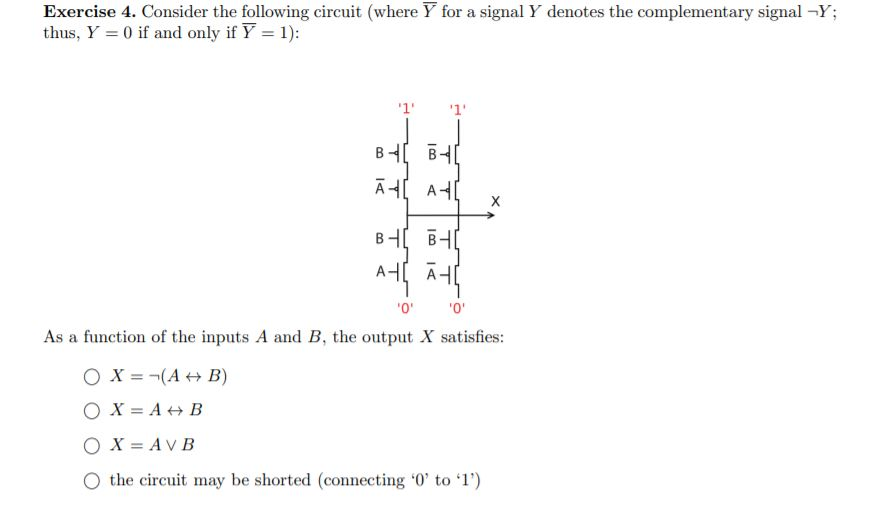
\includegraphics[scale=0.7]{epflLectureNotes/advancedComputation/figures/cmos2.JPG}
    \caption{PSET3 cmos problem}
    \label{fig:my_label}
\end{figure}

Here's how I solved it:
\\
Now notice that $X=1$ iff. $(B=0 \land \neg A = 0) \lor (\neg B = 0 \land A = 0)$ Thus we obtain:
\begin{align*}
    (\neg B \land A) \lor (B \land \neg A)\\
    \equiv \neg(B\lor \neg A) \lor \neg(\neg B \lor A)\\
    \equiv \neg(A \rightarrow B) \lor \neg(B \rightarrow A)\\
    \equiv \neg ((A \rightarrow B) \land (B \rightarrow A))\\
    \equiv \neg (A \iff B)
\end{align*}
\clearpage


And here is some more details on two's compliment:

\begin{figure}[H]
    \centering
    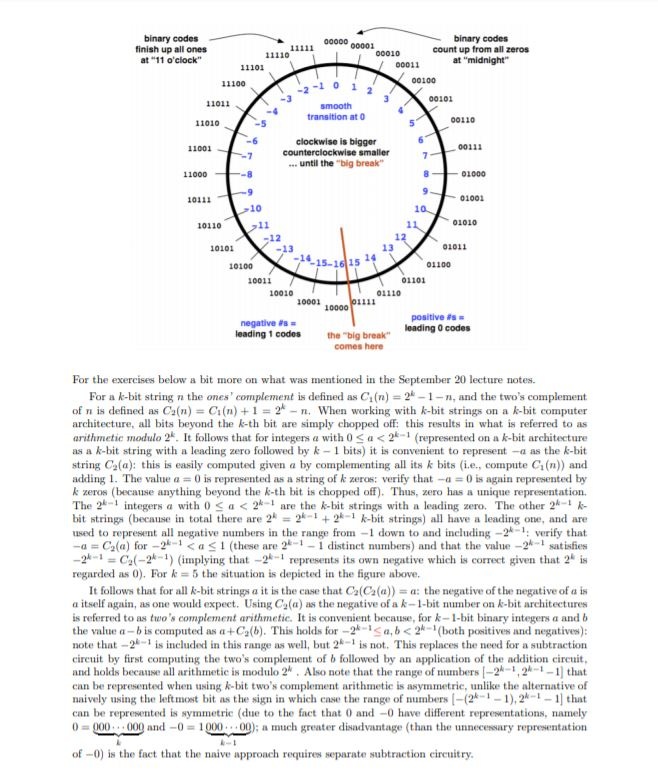
\includegraphics[scale = 1.2]{epflLectureNotes/advancedComputation/figures/twosc.JPG}
    \caption{More on two's compliment}
    \label{fig:my_label}
\end{figure}

And now let's say a little more about two's complement. That is, two's compliment simply represents the additive inverse of a number in $\bmod{2^k}$ That is, suppose we wanted some $b$ such that $a + b \equiv 0 \bmod{2^k}$, then we'd have that $b = 2^{k} - a$ Which is essentially the formula for two's complement for a given bit architecture. 


\subsection{Lec 07. notes}

We consider how to negate the $\exists!$ expression. Realize that:
$$\exists!xP(x) \equiv \exists x(P(x)\land P(y) \rightarrow (x=y))$$
And hence the negation(using our negation laws gives):
$$\neg\exists ! xP(x) \equiv P(x) \rightarrow \exists y \not = xP(y))$$
\\
And two demonstrate the importance of nesting order on quantifiers, consider this excerpt:

\begin{figure}[H]
    \centering
    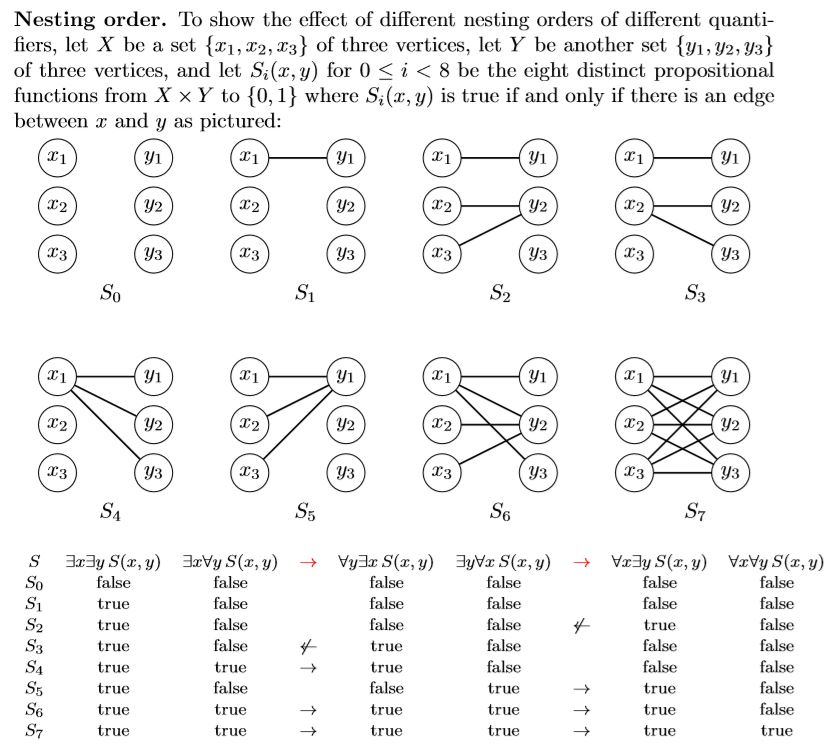
\includegraphics[scale = 0.8]{epflLectureNotes/advancedComputation/figures/nesting.JPG}
    \caption{Nesting order demo}
    \label{fig:my_label}
\end{figure}

And notice here how $\exists x \forall y S(x,y) \rightarrow \forall y \exists x S(x,y)$ This makes sense as whenever an x exists for each y, we have to have that for all y, there is an x. 
\\
\clearpage
And now we come to rules of inference for quantifiers. 

\begin{definition}(Inference laws for quantified statements)
\\
\textbf{Universal instantiation} 
\begin{equation*}
    \infer{P(c)}{\forall x P(x)}
\end{equation*}
\textbf{Universal generalization}
\begin{equation*}
        \infer{\forall x P(x)}{P(x) \text{for arbitrary x}}
\end{equation*}
And we note that the same hold respectively for the existential quantifier. 
\end{definition}

And finally we present an application of rules of inference. Suppose the following:
\\
$H(x):$ x is here
\\
$U(x):$ x likes C
\\
$L(x)$ x is a fan of D.R.(Denis Ritchie)
\\
Now we assert the following:
\\
(1) There is someone here who likes C
\\
(2) Everyone who likes C is a fan of D.R.
\\
Hence we get:
$$(1) \equiv \exists x(H(x) \land U(x))$$
$$(2) \equiv \forall x(U(x) \rightarrow L(x))$$
Now what may we infer from these?
\\
Well we know  $\exists x(H(x) \land U(x))$ hence we by instantiation we have $H(c) \land U(c)$ then $U(c),H(c)$ and since $ \forall x(U(x) \rightarrow L(x))$ to give $U(c) \rightarrow L(c), L(c)$ and finally $$H(c)\land L(c)$$
\\
And although it is not too useful to memorize their names, we include here a table of common rules of inference: 


\begin{figure}[H]
    \centering
    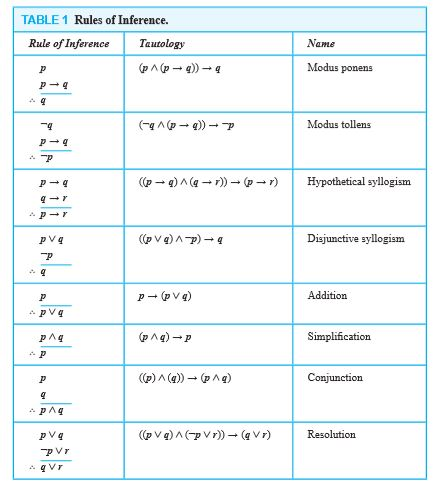
\includegraphics[scale = 0.9]{epflLectureNotes/advancedComputation/figures/inference.JPG}
    \caption{Rules of inference}
\end{figure}

\subsection{Lec 08. notes}
\subsubsection{Proof methods}
A \textbf{proof} is a valid argument establishing the truth of a statement. 
\\
We list some common proof methods and elaborate:
\\
\textbf{Direct proof:} When trying to prove a statement like $p \rightarrow q$ we consider the only case that $p \rightarrow q$ would be false and show that it can not happen. That is we take $p$ true and using our inference laws, reach that $q$ must be true as well 
\\
\textbf{Proof by contraposition:} Since $p\rightarrow q \equiv \neg q \rightarrow \neg p$ we try to show that the contrapositive holds via a direct proof. And here's a mini-example: Consider the statement \textit{if $n$ is an integer then $3n+2$ is odd.} Now suppose $3n+2$ is even to give $3n+2 = 2k, \ k\in \mathbb{N}$ Then we have that $n=\frac{2k-2}{3}$ and taking $k=2$ suffices to show $n$ is not an integer. 
\\
\textbf{Proof by contradiction:} Firstly, proof by contradiction is often confused with proof by contraposition. We use proof by contradiction to show that a statement $p$ is true. To do this, if we can show that $\neg p \rightarrow q$ is true where $q$ is always false, we have that $\neg p$ is false hence $p$ true. A common example is showing that $\sqrt{2}$ is irrational. We take the negation of $p$ that $\sqrt{2}$ is rational and derive the contradiction that whenever we try to write $\sqrt{2} = \frac{z}{k}$ with $\gcd{z}{k} = 1$ that $\gcd{z}{k} = 1 \land \gcd{z}{k} \not = 1$ Thus the falsity of $p$ implies a contradiction(false value) showing that $p$ itself must be true. 
\\
Similarly suppose we have statement $p\equiv a \rightarrow b$. We know that $\neg p \rightarrow a \land \neg b$ and get that $a\land \neg b$ is always false showing that $p$ must be true. 
\subsubsection{Graphs and planarity}
\textbf{A planar} graph is one that can be drawn without overlapping edges. Now a planar graph does not imply that for all possible drawing, overlapping edges wont exist. It simply means that a drawing could be made without overlapping edges. Now the two most important facts of graphs are:

 
 \begin{tcolorbox}[drop shadow, title=($K_{3,3}$ and $K_{5}$ are not planar),lower separated=true]
    Now notice that each connection we make partitions the plane into an inner and outer side following the \textbf{Jordan theorem}. We find out that when it comes to drawing the last vertex for $K_{3,3}$, the edge is surrounded by 4 curves making it impossible to not cross a curve. 
    \tcblower
    \centering
        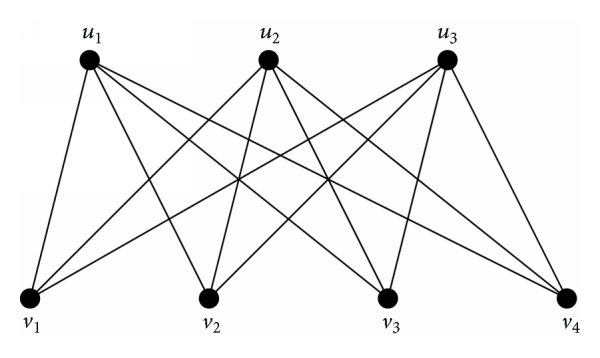
\includegraphics[scale = 1.1,valign=t]{epflLectureNotes/advancedComputation/figures/k3.png}
\end{tcolorbox}
\\
Now, \textbf{Kuratowski's theorem} states that a graph is non-planar iff it contains in one way $K_{3,3}$ or $K_{5}$
\clearpage
\subsubsection{Different surfaces}
We now consider different surfaces, those of the \textbf{Torus, Mobius strip, Klein bottle} shown respectively in the figure below. 

\begin{figure}[H]
    \centering
    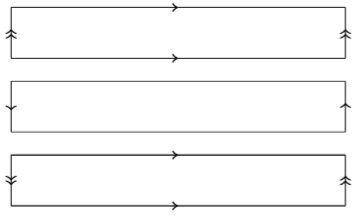
\includegraphics{epflLectureNotes/advancedComputation/figures/mobius.JPG}
    \caption{Rectangular abstraction}
\end{figure}

These surfaces are interesting because the laws of planarity no longer hold. For instance, on a mobius strip, $K_{3,3}$ is indeed planar as below. 

 \begin{tcolorbox}[drop shadow, title=($K_{3,3}$ has become planar),lower separated=true]
    \centering
        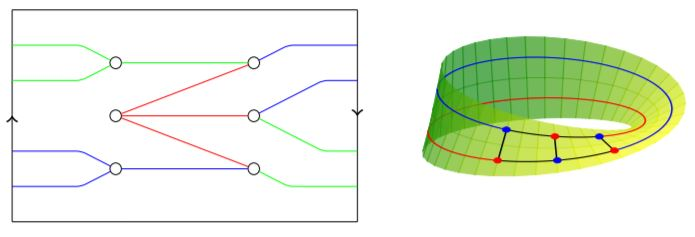
\includegraphics[scale = 0.9,valign=t]{epflLectureNotes/advancedComputation/figures/mobiusk3.JPG}
\end{tcolorbox}

\subsection{Lec 09. notes}
\subsubsection{Sequences}
We define a \textbf{sequence} as a mapping $f: \mathbb{N} \to \mathbb{R}$. Some most essential sequences are:

\begin{align*}
    \textbf{constant sequence} \ \exists c \forall i \ a_{i} = c\\
    \textbf{arithmetic sequence} \ \exists c \forall i \ a_{i+1} - a_{i}  = c\\
    \textbf{geometric sequence} \ \exists c \forall i \ \frac{a_{i+1}}{a_{i}}= c
\end{align*}
\\
More generally, the constant and arithmetic sequence are a member of the family of consecutive polynomial sequences. That is, since a polynomial is defines as:

$$\sum_{i=0}^{j} a_{i}X^{i}$$ we may have sequences of higher degree. 
\subsubsection{Summations}
Consider the summation of the first n terms of a constant sequence $a_{i} = c$. We would have $\sum_{i=1}^{n}a_{i}$ which is the same as $\sum_{i=1}^{n}c$ and taking $c=1$ we get n times 1 added which is $\sum_{i=1}^{n}c = 1$
\\
Let's now consider the summation of an arithmetic sequence by using an $nxn$ square as below: 
\begin{figure}[H]
    \centering
    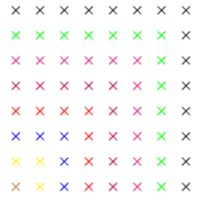
\includegraphics{epflLectureNotes/advancedComputation/figures/square.JPG}
    \caption{Summations, yey!}
\end{figure}

We agree that at each step there are $2i-1$ colored crosses which add up to $n^2$ many crosses. So we express it as $\sum_{i=1}^{n}(2i-1) = n^2$ and try to get a useful formula out of it. 
\\
Well we have that $\sum_{i=1}^{n}(2i-1) = \sum_{i=1}^{n}(2i) - \sum_{i=1}^{n}(1)$ Which further gives $2\sum_{i=1}^{n}(i) - \sum_{i=1}^{n}(1) = n^2$ hence we obtain $$\sum_{i=1}^{n}(i) = \frac{n^2 + n}{2}$$


\textcolor{gray}{We now consider more interesting summations involving} \textbf{telescoping sequences}. A telescoping sequence is a sequence where during summation of the terms (parts of) consecutive terms cancel each other, so that only few (parts of) terms remain to be added.
To illustrate this, consider the sequence $\{b_i\}$ for $i>0$ with $$b_i=i-(i-1),$$
and let $\{a_i\}$ be a constant sequence with $a_i=1$.
Obviously, it follows that $b_i=1$ so that $b_i=a_i$ and thus $\sum_{i=1}^nb_i=\sum_{i=1}^na_i$. The latter sum was already calculated, which was a trivial exercise but in principle still required adding together $n$ terms all equal to~1. Using that $\sum_{i=1}^nb_i=\sum_{i=1}^na_i$ the same sum $\sum_{i=1}^na_i$ can be computed by computing $\sum_{i=1}^nb_i$ instead: due to the telescoping effect, this computation does not require any actual calculations at all, but just involves careful administration:
\begin{eqnarray*}
\sum_{i=1}^nb_i&=&b_n\,+\,b_{n-1}\,+\,b_{n-2}\,+\,\ldots\,+\,b_2\,+\,b_1\\
&=&\underbrace{n-(n-1)}_{b_n}\,+\,\underbrace{n-1-(n-2)}_{b_{n-1}}\,+\,\underbrace{n-2-(n-3)}_{b_{n-2}}\,+\,\ldots\,+\,\underbrace{2-(2-1)}_{b_{2}}\,+\,\underbrace{1-(1-1)}_{b_{1}}\\
&=&n\underbrace{-(n-1)+n-1}_{=0}\underbrace{-(n-2)+n-2}_{=0}\underbrace{-(n-3)+\ldots}_{=0}\ldots\underbrace{\ldots+2}_{=0}\underbrace{-1+1}_{=0}\,-\,0\\
&=&n.
\end{eqnarray*}
\clearpage
Yet a much more formal way of showing this as follows:

\begin{eqnarray*}
\sum_{i=1}^nb_i&=&\sum_{i=1}^n(i-(i-1))\\
&=&\Big(\sum_{i=1}^ni\Big)-\Big(\sum_{i=1}^n(i-1)\Big)\,\,\,\,\text{     (in 2nd sum replace $i-1$ by $j$)} \\
&=&\Big(\sum_{i=1}^{n}i\Big)-\Big(\sum_{j=0}^{n-1}j\Big)\,\,\,\,\text{     (replace $j$ by $i$)} \\
&=&\Big(\sum_{i=1}^{n}i\Big)-\Big(\sum_{i=0}^{n-1}i\Big)\,\,\,\,\text{     (identify the part that occurs in both sums)} \\
&=&\Big(n+\sum_{i=1}^{n-1}i\Big)-\Big(0+\sum_{i=1}^{n-1}i\Big)\\
&=&n-0+\Big(\sum_{i=1}^{n-1}i\Big)-\Big(\sum_{i=1}^{n-1}i\Big)\\
&=&n.
\end{eqnarray*}

We now consider a different approach to geometric sequences. We are interested in a closed form expression for $\sum_{i=0}^ng_i$, where for relevant values of $r$ it may even make sense to talk about the value of $\sum_{i=0}^\infty g_i$.
Because $$\sum_{i=0}^ng_i=\sum_{i=0}^ng_0r^i=g_0\sum_{i=0}^nr^i$$
the value~$g_0$ is just an uninteresting multiplicative factor, and we omit it (i.e., from now on we assume that $g_0=1$; note that the entire sum equals zero if $g_0=0$).
Obviously, the problem is not interesting if $r=1$: then we get (with $g_0=1$) that
$$\sum_{i=0}^ng_i=\sum_{i=0}^nr^i=\sum_{i=0}^n1^i=\sum_{i=0}^n1=n+1.$$
Also $r=-1$ is not inspiring: we get 0 if $n$ is odd and 1 if $n$ is even; but the final arguments below work for $r=-1$ as well, so $r=-1$ is not excluded below.

Assuming $r\ne1$, we want to find a closed form expression for $\sum_{i=0}^nr^i$, i.e., for $$r^0+r^1+\ldots+r^{n-2}+r^{n-1}+r^n.$$
It was noted that we are already familiar with a similar sum, namely $$r^n+r^{n-1}+r^{n-2}+\ldots+r^1+r^0$$
which is just the same, but in the reverse order.
How come we are familiar with something like $r^n+r^{n-1}+r^{n-2}+\ldots+r^1+r^0$?
Just look at the decimal number $111\ldots11$ that consists of $n+1$ ones:
that is precisely the same as our expression $r^n+r^{n-1}+r^{n-2}+\ldots+r^1+r^0$ if we assume that $r=10$ (the \emph{basis} or \emph{radix} of our decimal number system) because our decimal number ${\color{red}{1}}{\color{green}{1}}{\color{blue}{1}}\ldots{\color{pink}{1}}{\color{magenta}{1}}$ is just a convenient shorthand notation for
$${\color{red}{1}}\times10^n+{\color{green}{1}}\times10^{n-1}+{\color{blue}{1}}\times10^{n-2}+\ldots+{\color{pink}{1}}\times10^1+{\color{magenta}{1}}\times10^0:$$
that is how the value of a number in decimal notation is defined, where the present case is particularly simple because all the digits are equal to one.

Taking for instance $n=4$, we find the number $11111$, and we know that if we multiply it by $9$ (which was carefully chosen as $10-1$, i.e., as $r-1$) we get, without any effort, $99999$, so that if we add one we get 100000, for which we have the nice closed form expression $10^5$ (i.e., $r^{n+1}$). We thus found that $$(11111\times 9)+1=10^5$$
and more in general that
$$(\underbrace{111\ldots11}_{n+1 \text{ ones}}\times 9)+1=10^{n+1},$$
or even more in general that
$$(\underbrace{111\ldots11}_{n+1 \text{ ones}}\times (r-1))+1=r^{n+1},$$
where the final $111\ldots11$ should be liberally interpreted as a shorthand notation for $r^n+r^{n-1}+r^{n-2}+\ldots+r^1+r^0$
and where we use that $10$ was just a placeholder for $r$ and thus that $9$ was a placeholder for $r-1$. This final expression leads us to believe that
$$\underline{(r^n+r^{n-1}+r^{n-2}+\ldots+r^1+r^0)\times(r-1)}+1=r^{n+1}$$
and thus that
$$r^n+r^{n-1}+r^{n-2}+\ldots+r^1+r^0=\frac{r^{n+1}-1}{r-1}$$
(where you should remember that indeed $r\ne 1$). But this is precisely the closed formula for $\sum_{i=0}^nr^i$ that we were trying to find, so we are done -- except we have not proved anything yet other than by intimidation.

To actually prove this result that
$$\sum_{i=0}^nr^i=\frac{r^{n+1}-1}{r-1}$$
if $r\ne 1$, have a look at the underlined part
$$(r^n+r^{n-1}+r^{n-2}+\ldots+r^1+r^0)\times(r-1)$$
of the equation above: 
apparently we need to prove that this underlined part is equal to $r^{n+1}-1$.
Pulling the factor $r-1$ inside the parentheses we get
$$(r-1)r^n+(r-1)r^{n-1}+(r-1)r^{n-2}+\ldots+(r-1)r^1+(r-1)r^0$$
and thus
$$r^{n+1}-r^n+r^n-r^{n-1}+r^{n-1}-r^{n-2}+\ldots+r^2-r^1+r^1-r^0.$$
\textcolor{gray}{This is yet another example of our earlier telescoping sum: all the intermediate terms cancel each other.}


In any case, the conclusion is that if $r\ne1$ then
$$\sum_{i=0}^nr^i=\frac{r^{n+1}-1}{r-1}$$
for any integer $n\ge0$.
It follows that if $|r|<1$ we have that
$$\sum_{i=0}^\infty r^i=\frac{1}{1-r}$$
because for $n\to\infty$ the term $r^{n+1}\to0$.
\\

We finally conclude by representing a useful identity as follows:

$$ \sum_{i=1}^{\infty}\sum_{j=1}^{i} \cdots =  \sum_{j=1}^{\infty}\sum_{i=j}^{\infty} \cdots$$
\clearpage

\subsubsection{Sum of $i^k$}
And yet another important point to mention is that all the sums of form $i^k$ may be found using the fact that the telescoping sequence given by $$f(k+1,i) = i^{k+1} - (i-1)^{k+1}$$ since using the telescoping property we have that $$\sum_{i=1}^{n} i^{k+1} - (i-1)^{k+1} = n^{k+1} $$ which means that $$\sum_{i=1}^{n} i^{k+1} = n^{k+1} + \sum_{i=1}^{n}(i-1)^{k+1} $$ where the $\sum_{i=1}^{n}(i-1)^{k+1}$ are recursively found. 


\subsubsection{Hilbert's Hotel}

Some interesting questions to pose on this matter are listed below with answers. 
\begin{question}
A bus carrying countably infinite number of guests arrives, can guests be accommodated? 
\end{question}
\begin{answer}
Well simply assign each former guest to odd numbered room and each new guest to even numbered room. 
\end{answer}

\begin{question}
Now suppose that countably infinite number of buses with countably infinite guests arrive what now?
\end{question}
\begin{answer}
Well, we move each guest in room $k$ to room $2k-1$. Now for new guests, $kth$ guest in bus 1 moves to $2^{1}(2k-1)$ hence in general $kth$ guest in bus $j$ moves to $2^{j}(2k-1)$ room. 
\end{answer}
\clearpage
\section{Algorithms and more (Week 5 - )}
\subsection{Lec 10. notes}
To demonstrate how summations come in handy consider snipets of following pseudocode


\begin{verbatim}
    B <- n while(B>0){step;} 
\end{verbatim}
Leads to $\infty$ steps.
\begin{lstlisting}
          B < - n while(B>0){for i=1 to B do step}){B = $\floor{\frac{B}{2}}$}
\end{lstlisting}
Now notice we first perform $n$, then approximately $\frac{n}{2}$ steps and so on. Thus in total we have $\sum_{i=0}^{\log_{2}{n} }(\frac{n}{2^j})$ many steps where this approximates to $2n$
\\
And now sum must now summation results:

\begin{figure}[H]
    \centering
    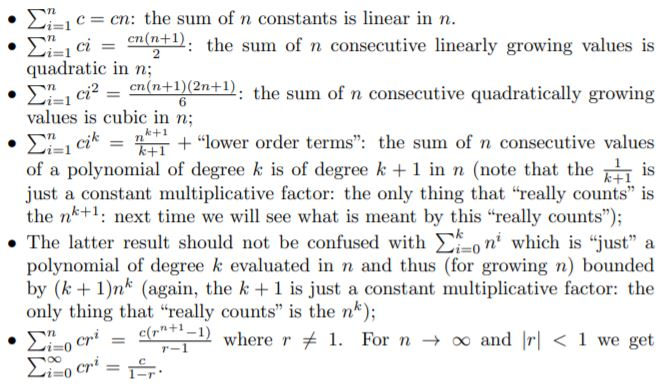
\includegraphics[scale = 0.7]{epflLectureNotes/advancedComputation/figures/sums.JPG}
    \caption{Summation formulae}
    \label{fig:my_label}
\end{figure}
And now we present \textbf{countability}:
\begin{definition} (Countabiltiy)
A set is countable iff. it is finite or there is a bijection from \mathbb{N} to the set. 
\end{definition}

And some countability facts:
\begin{itemize}
    \item Union of countable sets is countable
    \item \mathbb{Z} is countable, just map each odd number to the negative integers and each even number to positive integers. 
    \item Union of a finite number of countable sets is countable. That is for the finite $A_{k}$ $k$ many sets, first map all the $a_{0} \in A_{0}$ to 1, then $a_{1} \in A_{1}$ to 2 and hence $k+1 \to a_{1} \in A_{0} $
    \item Union of a countable number of countable sets is countable.
    \begin{figure}[H]
        \centering
        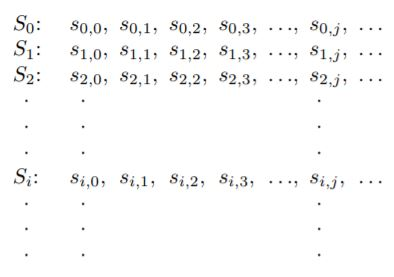
\includegraphics[scale = .6]{epflLectureNotes/advancedComputation/figures/walk.JPG}
        \caption{Enumeration}
        \label{fig:my_label}
    \end{figure}
    \item Cartesian product of two countable sets is countable (for which reason rational numbers are countable)
    \item Infinite union of bitsrings of finite length are countable. That is suppose we define $\bigcup_{i=0}^{j} S^{j}$ where $S = \{0,1\}$ Now $S^{0}$ has 1 element, $S^{1}$ has 1 distinct element, $S^{2}$ has 3 distinct elements and so on. Thus, we map $ 0 \to S^{0}$, then $1 \to 01 $ $2 \to 10$ $3 \to 11$. Since each $S^{k}$ has $2^{k}$ elements our mapping is defined. 
    \item The set $\{0,1\}^{*}$ consisting of infinite bitstrings is \textbf{uncountable} as follows by Cantor diagonilization. 
\end{itemize}
\\
A question from this week's pset asked:
\\
\begin{question}
Let $A$ be the set of real numbers with a finite number of 1 in the binary form and $B$ the set of all reals with a finite number of 1 in decimal form. Which of these sets is countable?
\end{question}
\begin{answer}
As it turns out, when we try enumerating members of A, we notice this is doable because for instance if we were to miss out enumerating one element it would have to be the case that it either contains a 0 which  we have already counted or a 1 which again we have already counted. Conversely for B, suppose we have enumerated all such numbers, but then define a new number with a digit differing in at least one decimal place of each element of B. 
\end{answer}

\subsection{Lec 11. notes}
We start with the \textbf{Halting problem} which states that given a computer program $P$ with input $I$ can we write a program that always determines whether $P(I)$ will terminate or not? As it turns out the answer is no.
\begin{example*}
Now let us define a program $A(P,x)$ that determines whether the program $P$ with input $x$ terminates. Now define $Q(x)$ as a program calling $A(x,x)$. Then $Q(P)$ runs $A(P,P)$ and $Q(P)$ will stop if $A(P,P)$ returns. Now consider $Q(Q)$. We have that $A(Q,Q)$ gets called. Well, if this returns no meaning $Q(Q)$ does not determinate, we get that $Q(Q)$ should terminate and vice versa. Hence, we get that such a program $A(x)$ can not exists. 
\end{example*}

\begin{definition}(Big $O$)
A function $f(x)$ is said to be $O(g(x))$ or informally $f$ is $O(g)$ if $$ \exists C,k \ \forall x>k, \ |f(x)| \leq C|g(x)|$$
\end{definition}


\begin{definition}(Big $\Omega$ )
A function $f(x)$ is said to be $\Omega(g(x))$ or informally $f$ is $O(g)$ if $$ \exists C,k \ \forall x>k, \ |f(x)| \qeq C|g(x)|$$
\end{definition}

\begin{definition}(Big $\Theta$)
if $f$ is both $O(g)$ and $\Omega(g)$, then f is $\Theta(g)$ meaning that f and g are of the same order
\end{definition}

\subsection{Lec 12. notes}

\subsubsection{Basics}
\textbf{Notion of Random access} We want our programs to have fast access to data. Thus an array is said to be \textbf{random access} if accessing or reading an element is independent of its index. Yet in reality this is far from true as there is only so much the \textbf{cache} can store. 
\\
When it comes to the cache, cache implements a compromise between spatial and temporal locality. That is, spatial locality refers to the likelihood that referencing a resource is high if something near it was referenced. Temporal locality refers to the notion that once a variable is called it will likely be called again. 
\\
An example is that Fortran caches 2-D arrays in column format. Hence to exploit spatial locality, when multiplying $A X B$ we would need to transpose $A$ and define matrix multiplication purely in terms of column to column inner products. 
\clearpage
\textbf{Binary search} When performing binary search on an ordered list, we let $m := \floor{\frac{n}{2}}$ for a list of $n$ items. Now whenever $l \not = l_{m}$ and our saught after element $l < l_{m}$ we reduce array size to range $l_{1}, .... , l_{m-1}$ and else to $l_{m+1}, .... , l_{n}$. Repeating the previous step, we obtain the in the worst case, we perform the floor operation until we reach the largest $k$ such that $\frac{n}{2^{k}} < 1$ to give us that $k$ which is how many steps we take is bounded by $\log_{2}n$ as $k < log_{2}n$
\subsubsection{Sorting algorithms}


\begin{tcolorbox}[drop shadow, title=(Overview of algorithms),lower separated=true]
\textbf{Bucket sort}
Simply arrange similar elements into buckets and the apply any sorting algorithm.
\\
\textbf{Bubble sort}
\begin{lstlisting}
    for(i = 1 to n-1){ if($l_{i}$ > $l_{i+1}$){.swap($l_{i},l_{i+1}$}}
\end{lstlisting}
The worst case is $\sum_{i=1}^{n} (n-i)$ swaps because for the largest element we have $(n-1)$ comparisons and swaps, for the second largest $(n-2)$ and so on which means that in the worst of cases we perform  $\sum_{i=1}^{n} (n-i)$ many operations which is $O(n^2)$. Now in the best case we have simply $n-1$ comparisons which is $\Omega(n)$
\\
\textbf{Selection sort}
To order in increasing order do: Locate smallest element in unsorted list and replace with first element in unsorted list. 
\\
\textbf{Insertion sort} Inserts $l_{2}$ in the right spot in the already sorted list $\{l_{1}\}$ and so on. Now at the $k^{\text{th}}$ step we have $\log_{2}(k)$ many comparisons using binary search. Hence total operations are bounded by $\sum_{k=1}^{n-1}(\log_{2}(k)$ comparisons. Insertion sort is $\Theta(n\log(n))$ if generally we use linked lists which prevent shifting problem present with arrays. 
\\
\textbf{Quick sort}
Take a pivot $l_{i}$ then create sublists $S_{1}$ of all smaller items and $S_{2}$ of all larger items. Then sort $S_{1}$ and $S_{2}$ using same method
\\
\textbf{Merge sort}
Treat each single element as a sorted list. Then take sublists of two elements and sort. Then merge each sublist making sure the ordering. Each new sublist of 4 elements is merged again and so on. We have that there are in total $\log_{2}(n)$ sublists with at most n comparisons hence $\Theta(n\log_{2}(n))$
\\
\textbf{Heap sort}
Create a tree using the initial order elements are given in. Then transform tree into a heap(calling heapify) by replacing each heap-violating node with child-element. Once heap is obtained, swap the largest parent with lowest child. Add largest parent to end of sorted list. Repeat process until tree contains only one element. Heap sort is $\Theta(n\log_{2}(n))$
\end{tcolorbox}


\subsection{Lec 13. notes}
\subsubsection{Some problems}
We begin with an interesting theorem. Given that $g_{1}$ and $g_{2}$ for $g_{i}: \mathbb{N} \to \mathbb{R^{*}_{+}$} and $f:\mathbb{N} \to \mathbb{R^{*}_{+}}$ are $\Theta(f)$ we want to show that $g_{1} + g_{2}$ is $\Theta(f)$ Now we know that:

$$ \exists k_{i},C_{i,n} \ \forall x > k_{i} \ C_{1,1}|f(x)| \leq |g_{1}(x)| \leq C_{1,2}|f(x)|$$ 
and :
$$ \ C_{2,1}|f(x)| \leq |g_{2}(x)| \leq C_{2,2}|f(x)|$$

Now seeing that $g_{1}(x) + g_{2}(x)$ is $O(f)$ is easy since $|g_{1}(x)| + |g_{2}(x)| \geq |g_{1}(x) + g_{2}(x)|$ which when we add our inequalities we obtain:

$$|g_{1}(x)| + |g_{2}(x)| \leq C_{1,2}+C_{2,2}(|f(x)|)$$ implying that $g_{1}(x) + g_{2}(x)$ is $O(f)$. For the $g_{1}(x) + g_{2}(x)$ is $\Omega(f)$ part, we know that our functions have the natural numbers as a domain which means that $|g_{1})(x)| + |g_{2}(x)| = g_{1}(x) + g_{2}(x)$ and since $C_{1,1}+C_{2,1}(|f(x)|) \leq |g_{1})(x)| + |g_{2}(x)|$ we have that $g_{1}(x) + g_{2}(x)$ is $\Omega(f)$. Yet this proof also shows that in general \textbf{$g_{1} + g_{2}$ is not $\Theta(f)$}. For instance when the $g_{i}: \mathbb{N} \to \mathbb{R}$ it is not always true that $g_{1} + g_{2}$ is not $\Theta(f)$.

\begin{example}
Let $g_{1}(x) = - g_{2}(x)$. Then we have that $g_{1} + g_{2} = 0 < c|f(x)|$ which as a consequence shows that $g_{1} + g_{2}$ is not $\Theta(f)$
\end{example}


\begin{example}
We now consider how to pin down the complexity of a given program. Suppose we are given:

\begin{lstlisting}
    for i=1 to n
        for j=1 to $\floor{\frac{n}{2}}$
            x = x + 1;
\end{lstlisting}

Now looking at the inner loop we see that it yields $\sum_{j=1}^{\frac{n}{2}} 1$ steps at most. And the two loops combined therefore yield $$\sum_{i=1}^{n}\sum_{j=1}^{\frac{n}{2}} 1$$ which is equal to:

$$\sum_{i=1}^{n} (\frac{i}{2}) = \frac{1}{4} n^{2} + n $$
\end{example}

\subsubsection{More complexity stuff}
An equivalent definition to Big-O is in terms of limsup as:

$$ f \text{is }O(g) \iff \limsup_{x\to\infty}{\frac{|f(x)|}{|g(x)|}} < \infty  $$

Which simply means that after some arbitrarily large $x$, f must increase at a lower rate than $g(x)$. Thus this definition may be used in showing that the witnesses exist. 
\\
And yet another complexity definition is:
\begin{definition}
$f$ is $o(g)$ (read f is little-o) whenever:
$$ \forall C > 0, \ \exists k \ \forall x>k, \ |f(x)| < C|g(x)|$$ Or equivalently:

$$ \lim_{x\to\infty}\frac{f(x)}{g(x)} = 0$$

\textit{We note that $f$ is $o(g)$ implies that $f$ is $O(g)$ as we may simply use universal instantiation to see this.}
\end{definition}
\\
\textbf{Fixed powers} For all positive constants $d,l$ we have that if $d \geq l$ then $n^l$ is $O(n^d)$ since $\limsup{\frac{n^l}{n^d}} < 1$.
\\

\textbf{Polynomials} For some polynomial $f(x)$ of degree $n$ such that:

$$ f(x) = \sum_{i=0}^{n}a_{i}x^{i}$$ we have that $f is O(x^{i})$ This may be seen since $f(x) \leq a_{max}x^{0} + \ldots + a_{max}x^{n} \leq a_{max}(d+1)x^{n} (\forall x > 1)$
\\

\textbf{Exponentials} Now for some exponential $S(n)$ such that: $$ S(n) = \sum_{i=0}^{n}a_{i}i^{d} $$
We have that each term is at most as big as $a_{max}n^{d}$ and with $n$ many such terms we have that $S(n) \leq na_{max}n^{d} = a_{max}n^{d+1}$ hence $S$ is $O(n^{d+1})$.
\\

\textbf{Powers of logarithms} (Note that this argument works for logarithms of any base). Suppose $f(x) = (\log(x)^t$ where t is a constant. Then $f$ is $O(n^{\epsilon})$ where $\epsilon$ is any real number larger than 0. 
\\
\textbf{More on logarithms} For constant $\sigma$ it is the case that $\log(n^\sigma)$ is $O(\log(n))$ and this is never the case without logarithms!
\\
We also have that for constant $\Gamma$ and $\sigma$ and whenever $a>b>1$ we have that $\log_{b}(x^{\sigma})$ is $O(\log_{a}x^{\Gamma})$ and not the other way around. We also have that for any $a,\Gamma > 1$ $\log_{a}(x^{\Gamma}$ is $O(\log(X)$ which may be seen via change of base. 
\\

\begin{tcolorbox}[drop shadow, title=(Properties and non-properties of big-O),lower separated=true]
{\bf{Properties and non-properties of big-$O$}} Let $f_i$ and $g_i$ be functions such that $f_i$ is $O(g_i)$ for $i=1,2$. It is often assumed that if some standard operation (such as addition (where $(f_1+f_2)(x)=f_1(x)+f_2(x)$), multiplication (where $(f_1f_2)(x)=f_1(x)f_2(x)$), powering (where $2^{f_i}(x)=2^{f_i(x)}$), logarithm (where $(\log(f_i))(x)=\log(f_i(x))$) is applied to the $f_i$-functions, that then the resulting composed function is again the big-$O$ of the same composition of the $g_i$-functions.
\begin{description}
\item[Addition (wrong)] \textcolor{gray}{In general} it is not the case that the function $f_1+f_2$ is $O(g_1+g_2)$: take for instance $g_2=-g_1$. It is not hard to prove, however, that $(f_1+f_2)(x)$ is $O(\max(|g_1(x)|,|g_2(x)|)$ (use the triangle inequality $|x+y|\le|x|+|y|$ -- can you prove the triangle inequality?).
\item[Multiplication (exceptionally correct)] It is true (and it is not hard to prove) that the function $f_1f_2$ is $O(g_1g_2)$.
\item[Powering (wrong)] In general it is not the case that $2^{f_1}$ is $O(2^{g_1})$: take for instance $f_1(x)=2x$ and $g_1(x)=x$, then $f_1$ is $O(g_1)$ (witness $C=2$), but $$\frac{2^{f_1}(x)}{2^{g_1}(x)}=\frac{2^{f_1(x)}}{2^{g_1(x)}}=\frac{2^{2x}}{2^x}=2^x$$
and $2^x$ can obviously not be bounded by any constant (for $x$ going to infinity) as would be required by $2^{f_1}$ being $O(2^{g_1})$ (remember the equivalence of ``$f$ is $O(g)$'' and $\limsup_{x\to\infty}\frac{|f(x)|}{|g(x)|}<\infty$:
because $\limsup_{x\to\infty}\frac{|2^{f_1}(x)|}{|2^{g_1}(x)|}=\infty$ it is not the case that $2^{f_1}$ is $O(2^{g_1})$).
Note that an incorrect answer is given to exercise 29 of Section 3.2 of the seventh edition of the book.
In the eighth edition it is exercise 42 in Section 3.2.
\item[Logarithm (wrong)] In general $\log(f_1)$ is not $O(\log(g_1))$. All we know about $f_1$ and $g_1$ is that there is a positive constant~$C$ (say $C>2$) such that for all large enough $x$ it is the case that $|f_1(x)|\le C|g_1(x)|$. It follows that $\log(|f_1(x)|)\le\log(C)+\log(|g_1(x)|)$, but that does not imply $|\log(f_1(x))|<\tilde C|\log(g_1(x))|$ for some constant $\tilde C$ and large enough $x$, as required for $\log(f_1)$ being $O(\log(g_1))$. If $f_1$ and $g_1$ are increasing and unbounded it follows that $f_1(x)>1$ and $g_1(x)>1$ for all $x>y$ for some $y$, so that logarithm-accidents involving huge negative values are avoided and we have $\log(f_1(x))\le\log(C)+\log(g_1(x))= \log(C)\frac{\log(g_1(x))}{\log(g_1(x))}+\log(g_1(x))$ and thus, using again that $g_1$ is  increasing, that $\log(f_1(x))\le\log(C)\frac{\log(g_1(x))}{\log(g_1(y))}+\log(g_1(x))\le\tilde C\log(g_1(x))$, where $\tilde C=\frac{\log(C)}{\log(g_1(y))}+1$. 
\item[Little-$o$ properties] Assume that $f$ is $o(g)$. Not only does this not imply $2^f$ is $o(2^g)$ (example: take $f(x)=\frac1{x^2}$ and $g(x)=\frac1x$) but neither does it imply that $\log(f)$ is $o(\log(g))$ (example: take $f(x)=x$, $g(x)=x^2$).
Addition and multiplication properties are maintained \textcolor{gray}{though.}
\end{description} 
\end{tcolorbox}
\\
\clearpage


\textbf{\textcolor{gray}{Symmetries and lack thereof}}
It is obvious that $f$ is $O(f)$ (but, as seen above, $f$ is not $o(f)$).
Generally speaking ``$f$ is not $O(g)$'' does not imply ``$g$ is $O(f)$'': indeed, functions $f$ and $g$ can be constructed such that it is not the case that $f$ is $O(g)$ and it is not the case that $g$ is $O(f)$. A dull example is $f(x)=\sin(x)$ and $g(x)=\cos(x)$; more interesting examples would be where both $f$ and $g$ are strictly increasing functions (cf. this week's exercises).

Note that if $f$ is $O(g)$ it may be the case that $g$ is $O(f)$ as well or it may be the case that $g$ is not $O(f)$.
The negation of $f$ is $O(g)$, i.e., ``it is not the case that $f$ is~$O(g)$'' or equivalently ``$f$ is not $O(g)$'', immediately follows from the above definition of big-$O$:
$$\text{``}f\text{ is not }O(g)\text{'' is equivalent to: }\,\,\,\,\,\,\,\,\,\forall\, C, k\,\,\,\exists x>k\,\,\,|f(x)|> C|g(x)|.$$
Thus, an ``occasional $x$'' (i.e., {\bf not necessarily all} $x$) that breaks the ``$\le$'' as required by big-$O$ suffices to negate $f$ is $O(g)$.
It follows that {\color{red}{to prove that $f$ is not $O(g)$ it suffices to find, for any constants $C>0$ and $k$, \underline{some} $x>k$ (not necessarily \underline{all} $x>k$) for which $|f(x)/g(x)| >C$}}.\\
\par\noindent
{\bf{The big-$O$ hierarchy}}
You should be familiar with the following underlined (and strictly increasing) \emph{hierarchy} of big-$O$s (and with the proofs: look at the ratios and consider the behavior for $n$ going to infinity, cf. $\limsup$-equivalence), where $b>1$, $\epsilon$ with $0<\epsilon<1$, $k>0$, and $d>1$ are fixed constants:
\begin{tabbing}
$\,\,\,\,\,\,\,\,\,\,\,\,\,\,$\=$\bullet$ {\color{purple}{any constant is$\,\,\,\,\,\,\,\,\,\,\,$}}\={\color{purple}{$\underline{O(1)}$}}\\
\>$\bullet$ {\color{purple}{$1$ is}}\>{\color{purple}{$\underline{O(\log(\log(n)))}\,\,\,\,\,\,\,$}}\={\color{red}{but $\log(\log(n))$ is not $O(1)$}}\\
\>$\bullet$ {\color{purple}{$\log(\log(n))$ is}}\>{\color{purple}{$\underline{O(\log(n))}\,\,\,\,\,\,\,\,\,\,\,\,\,\,\,\,\,\,\,$}}\={\color{red}{but $\log(n)$ is not $O(\log(\log(n)))$}}\\
\>$\bullet$ {\color{purple}{$(\log(n))^k$ is}}\>{\color{purple}{\underline{$O(n^\epsilon)$}}}\>{\color{red}{but $n^\epsilon$ is not $O((\log(n))^k)$}}\\
\>$\bullet$ {\color{purple}{$n^\epsilon$ is}}\>{\color{purple}{\underline{$O(n)$}}}\>{\color{red}{but $n$ is not $O(n^\epsilon)$}}\\
\>$\bullet$ {\color{purple}{$n$ is}}\>{\color{purple}{\underline{$O(n\log(\log(n)))$}}}\>{\color{red}{but $n\log(\log(n))$ is not $O(n)$}}\\
\>$\bullet$ {\color{purple}{$n\log(\log(n))$ is}}\>{\color{purple}{\underline{$O(n\log(n))$}}}\>{\color{red}{but $n\log(n)$ is not $O(n\log(\log(n)))$}}\\
\>$\bullet$ {\color{purple}{$n(\log(n))^k$ is}}\>{\color{purple}{\underline{$O(n^{d})$}}}\>{\color{red}{but $n^{d}$ is not $O(n(\log(n))^k)$}}\\
\>$\bullet$ {\color{purple}{$n^{d}$}} is\>{\color{blue}{\underline{$O(b^n)$}}}\>{\color{red}{but $b^n$ is not $O(n^{d})$}} \\
\>$\bullet$ {\color{blue}{$b^n$ is}}\>{\color{blue}{\underline{$O(n!)$}}}\>{\color{red}{but $n!$ is not $O(b^n)$}}\\
\>$\bullet$ {\color{blue}{$n!$ is}}\>{\color{blue}{\underline{$O(n^n)$}}}\>{\color{red}{but $n^n$ is not $O(n!)$}}, \=whereas {\color{magenta}{$n^n$ \underline{\bf is} $O((n!)^2)$}}\\
\>$\bullet$ {\color{purple}{$\log(n!)$ is}}\>{\color{purple}{$O(\log(n^n))$}}\>\>{\color{magenta}{\underline{\bf and} $\log(n^n)$ is $O(\log(n!))$}}\\
\end{tabbing}
To prove the statements about $n^d$ versus $b^n$ use $n^d=b^{d\log_b(n)}$ and observe that the latter's logarithmic in $n$ exponent $d\log_b(n)$ grows much slower than the exponent $n$ of~$b^n$.

From {\color{blue}{$n!$}} is {\color{blue}{$O(n^n)$}} (and the earlier discussion on logarithms) it follows that {\color{purple}{$\log(n!)$}} is {\color{purple}{$O(\log(n^n))=O(n\log(n))$}}. Conversely, from the fact that {\color{blue}{$n^n$}} is {\color{blue}{$O((n!)^2)$}} (this follows from $n^n\le(n!)^2$, which is easily seen to be the case\footnote{
Because $(n!)^2=\prod_{i=1}^ni(n-i+1)$, to prove that $n^n\le(n!)^2$ it suffices to prove that $n\le i(n-i+1)$ for $1\le i\le n$. This follows from the fact that the parabola $-i^2+i(n+1)-n$ is zero for $i=1,n$ and positive on the interval $1<i<n$.
%\vspace{10pt}\begin{tikzpicture}[scale=0.09]
%\draw (-1,0) -- (6,0);%node[pos=0.09]{1} node[pos=0.36]{$n$}; 
%\draw (0,-4.5) -- (0,2.5);
%\draw [black, thick, domain=0:5] plot (\x, {-4+5*\x-\x*\x});
%\end{tikzpicture}
}) it follows that {\color{purple}{$\log(n^n)=n\log(n)$}} is {\color{purple}{$O(\log((n!)^2))=O(\log(n!))$}}. We conclude that  {\color{purple}{$n\log(n)$}} is {\color{purple}{$\Theta(\log(n!))$}}.
Here everything in {\color{purple}{purple}} is called \emph{polynomial time} --- traditionally ``good'' --- and blue is \emph{exponential time} or worse --- traditionally ``bad''.\\
\par\noindent
\vspace{2pt}
\par\noindent
{\bf{Computational complexity}}
As we have seen during the lectures, the big-$O$ notation is a succinct way to catch the essence of the number of operations to be carried out by an algorithm to solve a certain problem.
Here it is assumed that a ``problem'' is interpreted as an infinite set of problem instances, where each problem instance has a certain well defined size.
For instance: ``sorting integers'' is a problem, and any integer sequence of length $n$ may be regarded as an instance of length~$n$ of the sorting integers problem; ``integer addition'' and ``integer multiplication'' are problems and any pair of $n$-bit integers may be regarded as an instance of length $n$ of the integer addition or of the integer multiplication problem.
Any instance of length $n$ of the sorting problem can be solved in time $O(n\log(n))$, any instance of length $n$ of the integer addition problem can be solved in time $O(n)$, any instance of length $n$ of the integer multiplication problem can be solved in time $O(n^2)$ using schoolbook multiplication, in time $O(n^{\log_2(3)})$ using Karatsuba multiplication. Since earlier this year it is known that it can be done in time $O(n\log(n))$ (Harley and van der Hoeven, cf. September 27 lecture notes). No one knows if multiplication can be done faster. 

We refer to the expressions in the big-$O$'s as the ``complexity'' (or ``time complexity'', or ``computational complexity'') of the problem at hand, or we say that the problem belongs to the ``complexity class'' $O(\ldots)$ for whatever $\ldots$ is applicable:
``the complexity of sorting is $n\log(n)$'', ``the complexity of addition is linear, but no one knows yet what the complexity is of multiplication''\footnote{Observe that each $\delta,k\in{\bf R}_{>0}$ gives rise to unique complexity classes $O(n^\delta)$, $O((\log(n))^k)$, and $O(n^\delta(\log(n))^k)$ and thus that there are uncountably many different complexity classes.}. Below a few common complexity classes are listed (where the $O$s may be replaced by $\Theta$s, except it is more common to use $O$s), along with common problems that belong to that complexity class:
\begin{itemize}
\item $O(1)$ (``constant'') to retrieve the largest item in a sorted list of any size, or to compute the parity of a number given in its binary representation;
\item $O(\log(n))$ (``logarithmic'') for binary search in a sorted list of $n$ items (if the list allows random access, for whatever that is worth);
\item $O(n)$ (``linear'') for linear search in a list of $n$ items that is not necessarily sorted (requiring only sequential access);
\item $O(n\log(n))$ (``n log n'') to sort a list of $n$ items using merge sort or heapsort\footnote{If we can only make ``binary decisions'' such as comparing items, we need at least $\log(n!)$ steps to be able to distinguish between all $n!$ possible distinct outcomes of the problem of sorting a list of $n$ items. Because $\log(n!)$ is of the same order as $n\log(n)$ sorting cannot be done faster than order $n\log(n)$.} but
\item $O(n^2)$ (``quadratic'') to do it using bubble sort or in the worst case of quick sort;
\item $O(n^3)$ (``cubic'') to multiply two $n\times n$ matrices (note that the input length in that case is $n^2$, so as a function of the input length it is ``only'' a degree $1.5$ algorithm and calling it cubic is a  bit misleading -- but traditional) and, a rather extreme example:
\item $O(n^{12})$ (``exponent twelve'') for the original 2002 AKS primality-proving method (``the three Indians method'' -- Indian indians, not American indians) to establish if an $n$-bit integer is prime or composite (this has in the meantime been improved to $O(n^6)$ (``exponent six'')). This should be contrasted with the ``practical'' method that does not give absolute certainty but that, for randomly generated numbers of hundreds of bits, has not failed yet and that runs in time $O(n^3)$ if schoolbook multiplication is uses (or $O(n^2\log(n))$ with the latest $O(n\log(n))$ multiplication method). 
\end{itemize}
\par\noindent
{\bf{The class {\bf P} of polynomial time solvable problems}}
Above we saw examples of problems that can be solved in time~$O(n^d)$, i.e., for which there exists an algorithm and a fixed constant $d$ such that for any problem instance of size~$n$ (i.e., the length of the input to the algorithm\footnote{In our input length estimates we disregard the sizes of the numbers involved. For the problems and algorithms considered in this course that will be adequate. For more complex problems a more precise approach must be used.}), the algorithm will produce a solution in a number of operations that is $O(n^d)$.
In the early 1970s it became customary to use the term \emph{polynomial time} for such algorithms.
If a problem can be solved by a polynomial time algorithm, the problem is polynomial time solvable (has \emph{polynomial complexity}), and the problem is said to belong to the class {\bf P} of polynomial time solvable problems:
{\color{red}{a problem~$X$ can be solved in polynomial time if there is an algorithm~$A$ and a fixed constant $d$ such that for all $n$ any instance of size~$n$ of problem~$X$ can be solved by~$A$ in $O(n^d)$ operations}}:
$$\exists A\,\exists d\,\forall n\,\forall {\text{ instances $I_n$ of size $n$ of $X$, $A$ solves $I_n$ in time $O(n^d)$}}. $$
Note the importance of the order of the quantified variables~$A$, $d$, $n$ and~$I_n$: reversing the order of the existentially quantified~$d$ and the universally quantified~$n$ and $I_n$ turns it into a useless property (it would always hold because it would become possible to choose~$d$ depending on~$n$ or $I_n$).

The existence of a polynomial time algorithm for a problem does not imply that each algorithm to solve the problem runs in polynomial time:
there are always plenty of ways to do things in a less clever manner that may take many more operations.
But, once a polynomial time algorithm for a problem has been found, the problem is, more or less and at least from a theoretical point of view, considered to be \emph{solved}, because it means that the number of operations required to find a solution can be nicely controlled by a ``decent'' polynomial function: of course solutions require more operations when larger problem instances are solved, but the growth of the number of operations is limited by a polynomial function and therefore thought to be reasonably well under control.

Everything that is purple in the ``big-$O$ hierarchy'' above is polynomial time, assuming that the input length is~$n$.
Problems in the class~{\bf P} are traditionally referred to as \emph{tractable} problems.
But notice that the fixed exponent $d$ in the expression that upper bounds the number of operations (up to a constant) may be \underline{any} nonnegative constant: one may wonder how ``tractable'' a polynomial time solution is for which $d=12$.

These nicely behaving polynomial time solvable problems are very much unlike nasty problems for which polynomial time solutions are not known to exist and for which the best algorithms known require at least \emph{exponential time}: the blue bulleted expressions in the ``big-$O$ hierarchy'' represent exponential time and worse (see below) run times, again assuming that the input length is~$n$.\\
\par\noindent
{\bf{Problems not known to be in {\bf{P}}}}
A simple example of a problem for which no polynomial time solution is known to exist is the knapsack problem: given a set~$S$ of $n$ items, each item in~$S$ with a value and a weight, the ``best'' subset of items in~$S$ must be found that satisfies a maximal weight restriction:
\begin{quote}
let $S=\{s_1,s_2,\ldots,s_n\}$ be some set of items, let $v, w: S\rightarrow{\bf R}_{\ge 0}$ be value ($v$) and weight ($w$) functions, and let $W\in{\bf R}_{\ge 0}$ be a maximal weight restriction. Find a subset $T\subseteq S$ such that $$\Big(\sum_{t\in T}v(t)\Big)\,\,\,\text{is maximized, while}\,\,\,\Big(\sum_{t\in T}w(t)\Big)\le W$$
\end{quote}
A solution would be to try all $2^n$ possible subsets $T$ of $S$ (while verifying the maximal weight $W$ restriction) and selecting the one of highest value, but~$2^n$ is exponential time.
It is often more convenient to replace the above \emph{optimization problem} by the --- mostly equivalent\footnote{Because the optimization problem can be solved by solving polynomially many decision problems (using binary search on potential $V$-values). The same comment applies to other optimization problems (such as traveling salesman or chromatic index).} --- \emph{decision problem} of deciding if for some specified value $V\in{\bf R}_{\ge 0}$ there exists a subset $T\subseteq S$ such that $\Big(\sum_{t\in T}v(t)\Big)\ge V$ and $\Big(\sum_{t\in T}w(t)\Big)\le W$ (and, if so, to provide such a subset~$T$).
Note that it can easily (i.e., in polynomial time, even in linear time) be checked if any proposed solution (i.e., some subset~$T$) to the latter decision problem is correct (i.e., satisfies the two conditions). How to efficiently construct such a solution, however, is unclear. In particular it is not known if exponential time is required.

Another example is the traveling salesman problem, where a bounded length tour must be found among $n$ cities: again a proposed solution can easily be checked, but finding one still escapes us, despite decades of intensive research.
Note that a solution can be found in $O(n!)$ operations by trying all possible tours.
Finding the chromatic index of a graph (the smallest number of colors required to color all vertices in the graph in a such a way that two neighbouring vertices have different colors) is -- for the moment at least -- not doable in polynomial time either; but checking if a given coloring satisfies a given bound is easily done (i.e., in polynomial time).
These examples should be contrasted with problem such as ``minimal spanning tree'' or ``shortest path'' which are both easily solvable in polynomial time: minimal spanning tree even by a greedy algorithm that consistently selects a new edge of lowest weight without closing a cycle.\\
\par\noindent
{\bf{The class {\bf{NP}}, and {\bf{P}} versus {\bf{NP}}}}
Occasionally a polynomial time solution is found for one of the nasty problems, but after a promising start in the 1970s this soon happened less and less frequently (once the low-hanging fruit was gone) and occurs only very rarely these days (this should not be interpreted as a reason to stop looking!).
The separation between the polynomial time solvable problems and those for which a polynomial time solution is not known to exist (yet?) persists to the present day.
A particular question that is found to be of interest (and that will earn you a one million US\$ prize if you solve it) is the {\bf P} versus {\bf NP} problem, namely if {\bf P} is properly contained in {\bf NP} or if {\bf P} and {\bf NP} are the same.
But, what is {\bf NP}? Probably not what you think it is, as explained in the next paragraph.

{\color{red}{The class {\bf NP} consists of those problems for which the correctness of a proposed solution can be verified in polynomial time}}: for instance, the decision versions of the knapsack and traveling salesman problems belong to {\bf NP}.
Note that {\bf NP} {\bf does not stand for ``not-P''}: it refers to the class of algorithms that can be solved in \emph{{\color{red}{n}}ondeterministic {\color{red}{p}}olynomial time}.
Here ``nondeterminism'' refers to the unspecified way in which a proposed solution is found: it may have been found by guesswork or any other way one sees fit (for instance, a ``nondeterministic'' one).

The difference between {\bf P} and {\bf NP} is the same as the difference between {\bf finding} a solution to a problem (namely in polynomial time) and {\bf verifying} (in polynomial time) that a given solution is correct -- without worrying at all in the latter case how the solution was found.
It is clear that all problems that belong to {\bf P} also belong to {\bf NP}.
It has not been proved yet that there are problems that belong to {\bf NP} but for which no polynomial time solution can exist (which would prove that {\bf P} $\ne$ {\bf NP} and thus that {\bf P} is properly contained in {\bf NP}) and neither has it been proved that all problems in {\bf NP} allow a polynomial time solution (which would prove that {\bf P} $=$ {\bf NP}).
Some argue that based on our failure to prove that {\bf P} $=$ {\bf NP}, despite the aforementioned decades of indeed intensive research, {\bf P} $\ne$ {\bf NP} is a safer bet than {\bf P} $=$ {\bf NP}.\\
\par\noindent
{\bf{NP-complete problems}}
The above statement ``neither has it been proved that {\color{red}{all}} problems in {\bf NP} allow a polynomial time solution'' sounds like a hopeless exercise, but this is what makes this field interesting:
it has been shown that there are problems in {\bf NP}, the so-called \emph{NP-complete problems}, that have the following intriguing property:
if a polynomial time solution is constructed for just a \underline{single} NP-complete problem (not for a single problem instance, of course...), then all problems in {\bf NP} are polynomial time solvable.
The first problem shown\footnote{Independently by two researchers in the very early 1970s: Stephen Cook and Leonard Levin.} to be NP-complete was the \emph{satisfiability problem} (finding an assignment of values to logical values such that a conjunction of disjunctions of the logical values (or their negations) evaluates to true), by showing that any problem~$X$ in {\bf NP} can be \emph{reduced in polynomial time} to the satisfiability problem (this means that solving~$X$ can be done in polynomial time, assuming the operations spent on solving one or more (but at most polynomially many) satisfiability problems are not counted). Other examples are the (decision versions of) the knapsack problem and the traveling \textbf{salesman problem.}

\subsection{Lec 14. notes}
\subsubsection{Mathematical induction}

Let's start by proving that mathematical induction is a valid proof technique.
In our proof we use the well-ordering principle which states that:

\begin{thm}
Every non-empty subset of the natural numbers contains a least element. 
\end{thm}

Let's now begin our proof:
\begin{proof}
Suppose that we have the statement $P(1)$ true and also that $P(k) \rightarrow P(k+1) \forall k \in \mathbb{N}$. Now also suppose that $\exists n \in \mathbb{N}$ for which $P(n)$ is false. Let now $S=\{\text{all indexes for which P(n) is false}\}$. Now by the well-ordering property we have that $S$ is non-empty. Let $m$ be the least element of $S$. Now $m$ can not be 1 since since $P(1)$ is true. Now notice that because $m$ is a positive integer greater than 1, we have that $m-1$ must be a positive integer that is not in $S$. Hence we have that $P(m-1)$ is true. Now by our induction hypothesis(which is also true) we have that $P(m)$ must be true. Hence we have that $P(n)$ is true for all $n$.
\end{proof}

\subsection{Lec. 15 notes}

\subsubsection{Worse than exponential time}
We note that $n!$ is worse than exponential time $b^d$. And now let's derive an expression for subexponential time complexity. That is we need a function that lies between $n^d$ and $b^n$ where $d,b$ are constants. We write $n^d$ as:
$$n^d = b^{(\log_{b}n)^{d}}$$
From this we note that the expression:
$$ b^{d\cdot n^{r}(\log_{b}n)^{1-r} $$ denotes subexponential time. The closer r is to 1, the closer we are to exponential time.
\\
Another function that lies between polynomial and exponential time is quasi-polynomial time. Consider the expression: 
$$ b^{(\log_{b}(n))^c}$$. For instance when $c=1$ we have $n^{log_{b}n}$ which is worse than polynomial time as the exponent grows and is unbounded. 

\subsubsection{Some exemplary proofs}

\begin{example}
We claim that any natural number greater than or equal to 8 can be represented as a combination of 3's and 5's.
\end{example}

\begin{proof}
We will use strong induction here(which we remind is equivalent to induction). Strong induction is the tautology that:
$$ P(0) \land \forall k[\forall l \leq k \ P(l) \rightarrow P(k+1)] \rightarrow \forall k P(k)$$
\\
Now our base case P(8) is clear. Let now $P(k-2)\land P(k-1)\land P(k)$ be our inductive hypothesis. We need to show $P(k+1)$. Well $P(k+1)$ clearly holds because given that $P(k-2)$ if we simply add 3 to the combination present in $P(k-2)$ we are done. Therefore we have shown that $P(k-2)\land P(k-1)\land P(k) \rightarrow P(k+1)$ is a tautology. And since we have that $P(8) \land P(9) \land P(10)$ as our basis step we are done.
\end{proof}

\subsection{Lec 16. Notes}

Consider the statement that everyone is equal. Let's tackle this with weak induction. 

\begin{example}
Now our statement says $P(n) \ \forall n \geq 1$ As a basis step we take $P(1)$ which is trivially true. Now assume $\forall k \ P(k)$ Then we get that $P(k+1)$ also holds because persons through $2 - k+1$ are the same(by IH) and persons through $1 - k$. Yet, the problem lies in our basis. That is $1$ person being the same does not imply that any two other persons are the same. 
\end{example}

\begin{example}
Suppose we claim that $p^2 + p + 1 | p^{n+1} + p^{2n-1} \ \forall n\geq1$ The basis $P(1)$ is trivial. Now assume $\forall k P(k)$ Then we have that $P(k+1)$ is:
$$p^2 + p + 1 | p^{n+2} + p^{2n+1}$$ Now we try to rewrite $p^{n+2} + p^{2n+1}$ as:
$ p(p^{n+1} + p^{2n-1}) + x $ where $x = (p^2 + p + 1)(p+1)^{2k-1}$ hence we are done.
\end{example}

\begin{example}
Consider the claim that every $ 2 \leq n\in \mathbb{Z}$ is divisible by a prime number. Basis is trivial. Now assume that $\forall l \ 2 \leq l \leq k P(l)$ Given this, for $P(k+1)$ we have that either $k+1$ is prime or that $k+1 = a\cdot b$ where both $a,b \leq k$ hence IH applies to both and we are done. 
\end{example}

And now we come to a more appealing example. 

\begin{example}
\label{exC}
We claim that a chocolate bar of $m$ single blocks can be broken into $m$ single blocks in $m-1$ breaks. Let's use strong induction again. Now base case $P(1)$ is trivial. Let now our IH be:
$$ \forall l, \ 1\leq l \leq k \ P(l)$$ Now given this consider we have a bar of $m-1$ blocks. Then suppose we break it into $m$ and $k+1 - m$ pieces at the cost of \textcolor{red}{1} break. Now our IH applies to both the blocks since their size is less than $m$. Through this we have that $m$ will take $m-1$ and $k+1-m$ will take $k+1-m-1$ steps which in total gives $m-1 + k+1-m-1 + 1 = k$ steps and we are done. 
\end{example}
\\ 
Let's now expand on example \ref{exC}. Suppose that instead of defining one single break as a cost of 1, the cost of breaking $m$ blocks into $m-L$ and $L$ blocks is defined as $L(m-L)$. Now our goal is to find the optimal cost and prove it. As an example if we break $n$ pieces into $n-L$ and $L$ many pieces than net cost is $L(n-L)$. Notice that we may define the total cost $S(n)$ of breaking $n$ pieces into $n$ single units recursively as:

$$ S(n) = \min_{1\leq k \leq n}(k(n-k) + S(n-k) + S(k))$$
Now we conjecture that $S(n) = \frac{n(n-1)}{2} \ \forall n \geq 1$

\begin{proof}
Basis is trivial. As for strong IH, we have that $$ \forall 1 \leq l \leq n, \ S(l) = \frac{l(l-1)}{2} $$ We now have to show that $S(k+1) = \frac{k(k+1)}{2}$ Now by definition we have that:
$$ S(k+1) = \min_{1\leq l \leq k+1}(l(k+1-L) + S(k+1-l) + S(l))$$ By our hypothesis and simplifications we get that $S(k+1) = \frac{(k+1)k}{2}$ as intended. 
\end{proof}

\begin{tcolorbox}[drop shadow, title=(Useful analogy),lower separated=true]
An intuition for our above result is the handshaking example. Suppose that a group of $n$ people split up into a group of $n-k$ and $k$ people. Hence at every splitting there are $(n-k)k$ handshakes. And at the end there are obviously $\underbrace{n-1 + n-2 + \ldots + 1}_{\text{each person is a node}}$ many handshakes which is equal to $\frac{n(n-1)}{2}(\text{by summation for arithmetic series})$
\end{tcolorbox}

\subsection{Lec 17. notes}
We come to the subject of recursion. Recursion is similar to induction in the way that it exploits a base step called "bottom of recursion". Let's first see examples of where recursion is hidden. 

\begin{example}
We may define summation $\sum_{i}^{u} x_{i}$ recursively as:

$$ \sum_{i}^{u-1} x_{i} + x_{u} \ \text{if $i \leq u$} \ \text{and if $i > u$} \sum_{i}^{u} x_{i} = 0$$
\end{example}

We may do the same for multiplication, that is:

\begin{example}
We define $\prod_{i}^{u} x_{i} $: 

$$ x_{u} \cdot \prod_{i}^{u-1}  \text{if $i\leq u$} \ \text{and else} \prod_{i}^{u} = 1$$
\end{example}

And notice that the above may be implemented programmatically:

\begin{lstlisting}
    sum(i,u,$x_{i}$) = if l>u then 0 else sum(i,u-1,$x_{i}$) + $x_{u}$
\end{lstlisting}

Similarly the factorial function is defined recursively as:
$$n! = n \cdot (n-1), \ 0!=1$$
\\

Now recursion becomes very useful for fast exponentiation. Observing the following:

$$ a^{171} = (a^{85})^{2} \cdot a = ((a^{42})^{2}\cdot a)^{2} \cdot a = \ldots$$

We define $p_{l}$ the exponentiation function as:

$$ p_{l}(a,l) = \text{if} \ n\leq 0 \ \text{then} 1\ \text{else} \ a^{n\text{&}1}\cdot p_{l}(a,\floor{\frac{n}{2}})^{2}$$ where $a^{n\text{&}1} = \{0,1\}$ and is equal to 1 iff n is even. 

















\end{document}
















